\documentclass[journal]{IEEEtran} 
\usepackage{cite,graphicx}
\usepackage{graphicx}
\usepackage{subfig}
\usepackage{wrapfig}
\usepackage[export]{adjustbox}
\usepackage{float}

\newcommand{\SPTITLE}{CREATING AN ARTIFICIAL GAME PLAYER FOR MODIFIED STICK RUNNING USING NEURO EVOLUTION OF AUGMENTING TOPOLOGIES (NEAT)}
\newcommand{\ADVISEE}{Aldrich S. Goco}
\newcommand{\ADVISER}{Rozano S. Maniaol}

\newcommand{\BSCS}{Bachelor of Science in Computer Science}
\newcommand{\ICS}{Institute of Computer Science}
\newcommand{\UPLB}{University of the Philippines Los Ba\~{n}os}
\newcommand{\REMARK}{\thanks{Presented to the Faculty of the \ICS, \UPLB\
                             in partial fulfillment of the requirements
                             for the Degree of \BSCS}}
        
\markboth{CMSC 190 Special Problem, \ICS}{}
\title{\SPTITLE}
\author{\ADVISEE~and~\ADVISER%
\REMARK
}

\IEEEpubid{\copyright~2020~ICS \UPLB}

%%%%%%%%%%%%%%%%%%%%%%%%%%%%%%%%%%%%%%%%%%%%%%%%%%%%%%%%%%%%%%%%%%%%%%%%%%

\begin{document}
\maketitle
\pagestyle{headings}

\begin{abstract}
In this work, an artificial game player for the Modified Stick Running was created using the NeuroEvolution of Augmenting Topologies (NEAT) algorithm. NEAT was used to evolve the neural network of the game agent to play the game indefinitely. Game states are represented using three features including the height and width of the nearest obstacle and also its distance to the game agent. The fitness of the agent is the combination of its score and traveled distance. The Algorithm was run for 30 trials with a maximum allowable generation of 30 and a maximum scoring of 50 points. The experiment has shown that the NEAT algorithm has a success rate of 83.33 percent and an average of breakthrough at 16.8 generations.
\end{abstract}

\section{INTRODUCTION}

\subsection{Background of the Study}

Stick Running is an endless running game platform game. It is a single player game wherein the human player controls the game character to jump in order to avoid all of the of the varying obstacles as the game character attempt to run as far as possible. Once the game character run into any obstacle then the game will be over. While it is relatively easy for a human player to learn basic strategy for Stick Running, it might be another story when it is played by an Artificial Intelligence (AI). The issue is that it is a challenge for a person to describe precisely their playing strategy, or to represent such a strategy formally (e.g., as a set of rules).

Fortunately, thanks to the advancement on Artificial Intelligence (AI) research, there are already existing methods such as Machine Learning (ML) that could address the said issue. One example of Machine Learning (ML) is the Neuroevolution of augmenting topologies (NEAT) which will be used in this paper to develop an artificial agent that replaces human in playing the Modified Stick Running.

Neuroevolution of Augmenting Topologies (NEAT) is an evolutionary computation method that evolves the topology and weights of an Artificial Neural Network (ANN) [1]. As such it represents an advance from methods that evolve only the weights of topologically fixed networks. Allowing NEAT to control the topology of the ANN gives it the power to scale the complexity of the network to match that of the problem - increasing the number of nodes for more complex problems and reducing it for less complex ones, in addition to simply adjusting connection weights. Additionally, NEAT attempts to balance the fitness of evolved solutions and their diversity. It is based on applying three key techniques: tracking genes with history markers to allow crossover among topologies, applying speciation to preserve innovations, and developing topologies incrementally from simple initial structures (i.e. complexication) [2].

\subsection{Significance of the Study}

Articial Intelligence (AI) can improve the daily quality of human lives. One example of those improvements, on the verge of becoming a daily reality, are self-driving cars [3]. Real-world problems such as this one are however a very difficult AI testbed. It is therefore very common that before trying to develop intelligent agents for real-world environments, we use synthetic and more controlled abstract environments. Game platforms, such as the one in this paper, are therefore almost ideal to develop methods and gain knowledge, providing the basis that can afterwards be applied on more dynamic and complex problems [4].

\subsection{Objectives of the Study}

The general objective of this study is to develop an agent capable of learning to play the game Modified Stick Running and survive indefinitely. Specifically, it aims to:

\begin{itemize}

\item Implement an Artificial Neural Network (ANN) to act as the brain of the game agent.
\item Implement the NeuroEvolution of Augmenting Topologies (NEAT) system for the training of the game agent.
\item Develop an evolved Game Agent that could survive fifty obstacles of seven variations by jumping over them

\end{itemize}

\IEEEpubidadjcol

\subsection{Scope and Limitations}

Since the focus of this study is the development of the Agent that will play the Modified Stick Running through the application of NeuroEvolution of Augmenting Topologies (NEAT), the aesthetics of the game itself will not be as fine-tuned compared to the original work. The landscape of the game is simplified into a non-changing flatland compared to the shifting one from the original work. The obstacles are also simplified into blocks or combination of blocks compared to the flying rockets, chainsaws and slanted wall in the original work.

\IEEEpubidadjcol

\section{REVIEW OF RELATED LITERATURE}

Machine Learning has played a part in the research for the development of Artificial Intelligence for Video Games. From the different types of Machine Learning used in Artificial Intelligence for Video Games there are two notable kinds who are popularly used, the Reinforcement Learning and the Genetic Algorithm [5].

Reinforcement learning, in the context of artificial intelligence, is a type of dynamic programming that trains algorithms using a system of reward and punishment. A reinforcement learning algorithm, or agent, learns by interacting with its environment. The agent receives rewards by performing correctly and penalties for performing incorrectly. The agent learns without intervention from a human by maximizing its reward and minimizing its penalty.

There are existing works about the application of reinforcement learning for a game agent. TD-gammon, a backgammon-playing program developed in 1990s, is one of the most successful example in reinforcement learning area. In [6], TD-gammon used a model-free reinforcement learning algorithm similar to Q-learning, and approximated the value function using a multi-layer perceptron with one hidden layer1. 

A team from Google’s DeepMind [7] developed a reinforcement learning
agent called deep Q network (DQN) that trains a deep convolutional ANN via
Q-learning. DQN managed to reach or exceed human-level playing performance in
29 out of 46 arcade (Atari 2600) games of the Arcade Learning Environment[8].

On the other hand, Genetic Algorithm makes uses of techniques inspired from evolutionary biology such as selection, mutation, inheritance and recombination to solve a problem. The most commonly employed method in genetic algorithms is to create a group of individuals randomly from a given population. The individuals thus formed are evaluated with the help of the evaluation function provided by the programmer. Individuals are then provided with a score which indirectly highlights the fitness to the given situation. The best two individuals are then used to create one or more offspring, after which random mutations are done on the offspring. Depending on the needs of the application, the procedure continues until an acceptable solution is derived or until a certain number of generations have passed.

The method that will be used in this paper, the NeuroEvolution of Augmenting Topologies (NEAT) is also categorized as a Genetic Algorithm, the only difference is the procedure on evolving a neural network. In NEAT, each individual represents a neural network or a genome. A sample neural network represented by an individual can be seen in Figure 1. Under the NEAT Genome, the node gene represent the node in the neural network while the connection gene represent the connection between two nodes and its weight. Connections might be enabled or disabled. NEAT keeps track of the structural changes with a number called innovation. Whenever a new connection is formed, they get a new incremented innovation number.

\begin{figure}[htbp]
    \begin{center}
        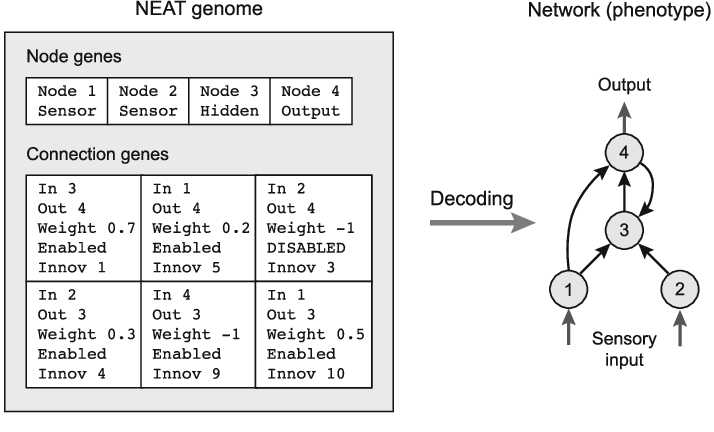
\includegraphics[width=8cm, height=6cm]{Genome.png}
        \caption{A sample Genome}
    \end{center}    
\end{figure}

This representation of the neural network of an individual by the NEAT is the key factor that made it an innovative neuroevolutionary algorithm for it eases the operations done in a genetic algorithm. The paper presented Stanley and Miikkulainen about NEAT explains in details on how it emulates the methods of a genetic algorithm. The following is the simplified version of the steps.

(1) Mutation Operation in NEAT can change both connection weights and network structures. Connection weights mutate as in any NeuroEvolution system, with each connection either perturbed or not at each generation. It can also be enable or disable connection. Structural mutations occur in two ways which can be seen in Figure 2.

\begin{figure}[htbp]
\begin{center}
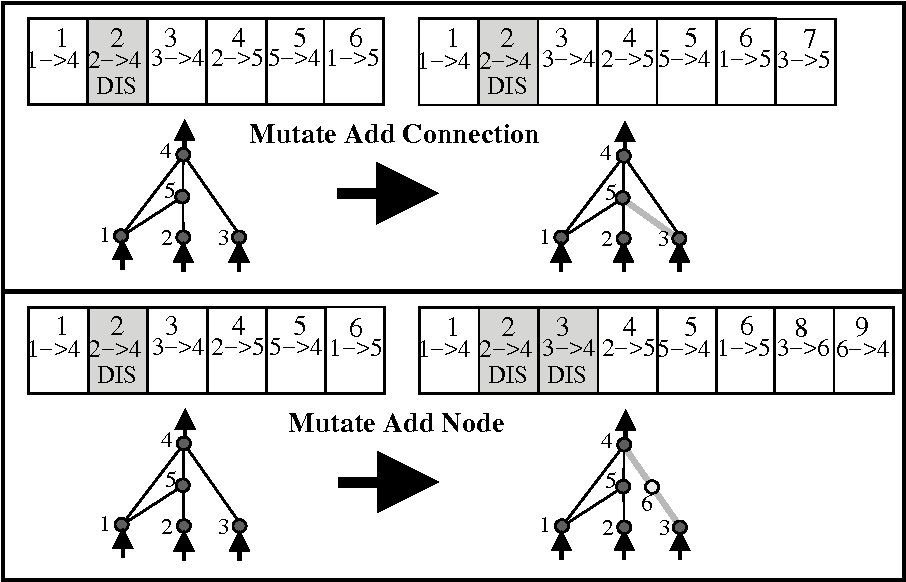
\includegraphics[width=8cm, height=6cm]{mutate.png}
\caption{The two types of structural mutation in NEAT}
\end{center}
\end{figure}

(2) Due to the implementation of Innovation marking, the crossover operation or exchange of genes can be done without structural analysis. An example can be seen in Figure 3.

\begin{figure}[htbp]
\begin{center}
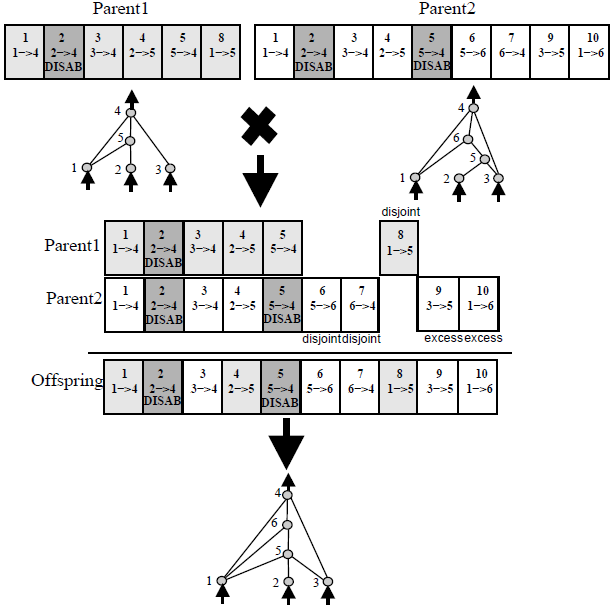
\includegraphics[width=8cm, height=6cm]{crossOver.png}
\caption{Matching Up Genomes for Different Network
Topologies Using Innovation Numbers}
\end{center}
\end{figure}

(3) Speciation is the process of grouping individuals whose genetic structure or topologies are closely related. Its organisms to compete primarily within their own niches instead of with the population at large. This way, topological innovations are protected in a new niche where they have time to optimize their structure through competition within the niche.

The uses of NEAT ranges from finding a Go player
agent independent on the board size [9], to use in realtime
environments such as Neuro-Evolving Robotic Operative
(NERO). In the latter case, it is called real-time
Neuroevolution of Augmenting Topologies (rt-NEAT) [10].
In a NERO context, NEAT is employed in the training of
groups of virtual robots capable of playing against other
teams. A very distant NEAT variation is content-generating
Neuro-Evolution of Augmenting Topologies (cg-NEAT) [11],
in which NEAT is used to generate the contents of a game
called Galatic Arms Race (GAR). It allows the game to
change during execution, increasing players’ immersion and
retaining their attention. We also call attention to NEAT’s
use in the development of playing agents for Fighting
Games, where building a consistent form of measuring
fitness is quite relevant [12].

NEAT can also be applied to the multiobjective paradigm
in certain games, where NPCs must perform more than one
task, such as Ms. Pac-Man [13].

\section{METHODOLOGY}

\subsection{Requirements}

The study will use the Neuroevolution of augmenting topologies (NEAT) python library that is available on the Github repository of CodeClaimers [14]. The Stick Running Game will be created using the PyGame library [15]. The development of the game and the implementation of the Neuroevolution of augmenting topologies (NEAT) to train the game agent will be done in a laptop with the following specifications:
CPU: Intel i3-8310U @2.2GHz processor
GPU: Nvidia GeForce MX150
RAM: 4.00GB RAM DDR4 
OS: Windows 10 Enterprise 64-bit

\subsection{Neural Network of Game Player}

Due to the nature of Neuroevolution of augmenting topologies (NEAT) of optimizing and complexifying from minimal structured neural network [1], the design of the Artificial Neural Network (ANN) would initially start from 3 input node which are connected to 1 output node with no hidden node, as shown in Figure 4b. The input layer or the sensors that were used were made up of the following 3 nodes:

\begin{itemize}
\item A: Distance of player to nearest obstacle
\item H: Height of the nearest obstacle
\item W: Width of the nearest obstacle
\end{itemize}

For supplying the controller with information about game states, internal game state variables were
directly accessed and fed as inputs to the neural network as shown in Figure 4a.

When the agent receives the information given by the
environment (A, H and W), it is processed by the network,
generating a probability of executing a jump. If the output is greater than 0.5 then the agent will jump, otherwise none will happen.

\begin{figure}[htbp]
    \begin{center}
        \subfloat[sensors in game]{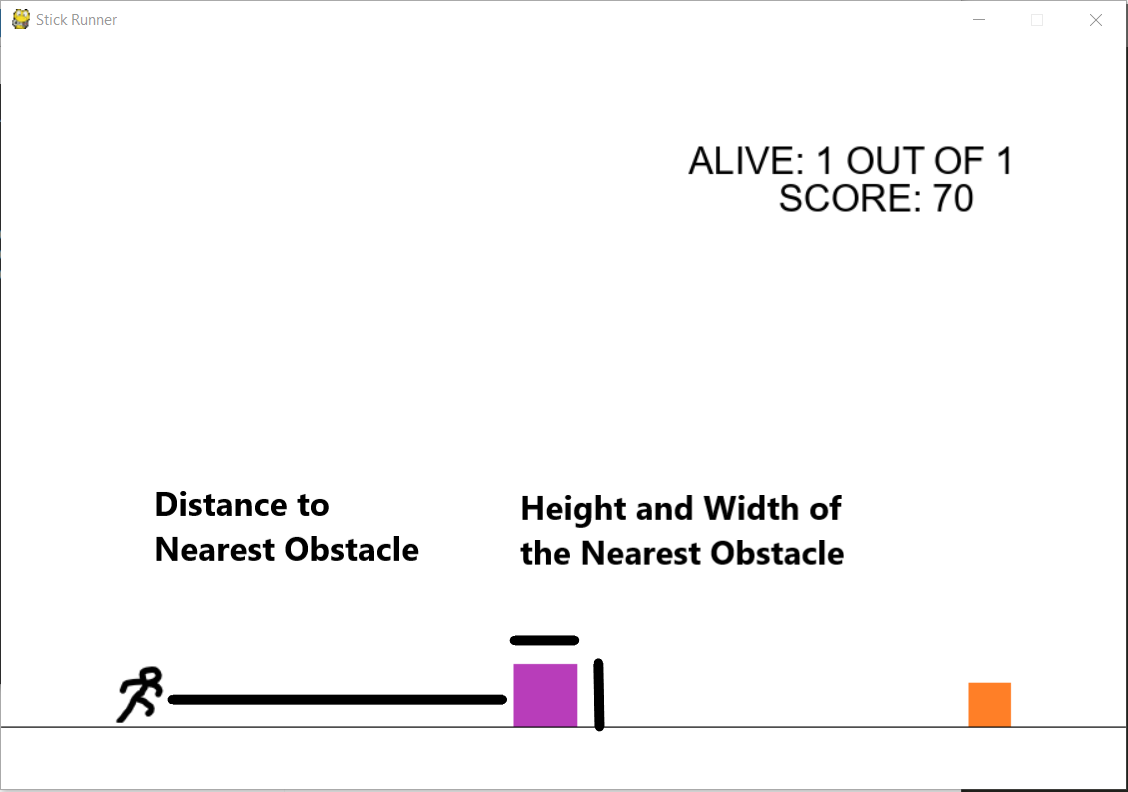
\includegraphics[width=6cm, height=4cm]{sampleImage1.png}}

        \subfloat[network architecture with unknown initial structure]{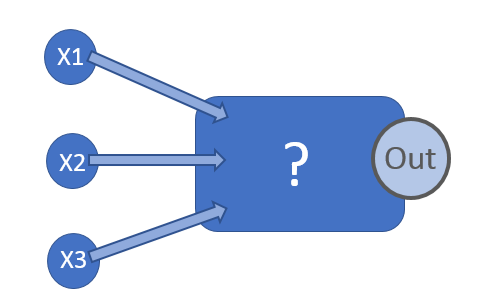
\includegraphics[width=6cm,height=4cm]{defaultGenome.png}}
    \end{center}
\caption{Different look at the genome representation}    
\end{figure}

\subsection{Game and Obstacles settings}

In the Modified Stick Running game, there are seven types of land obstacles that the player will encounter while running the game as shown in Figure 5 items which are:

\begin{itemize}
\item(a) Red: small width and small height 
\item(b) Orange: medium width and small height 
\item(c) Yellow: large width and height 
\item(d) Green: small width and medium height 
\item(e) Blue: medium width and medium height 
\item(f) Violet: large width and medium height 
\item(g) Black: small width and large height    
\end{itemize}

These seven obstacles then are randomly generated with a minimum gap of 300pixels to one another. Additionally, the obstacles and the players are moving at the same speed which were determined in the Game attributes.

\begin{figure}[htbp]
    \begin{center}
        \subfloat[]{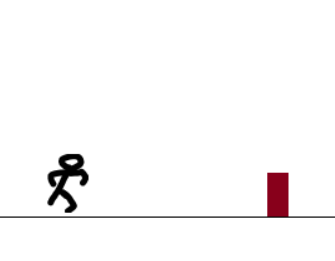
\includegraphics[width=2cm, height=2cm]{1b1.png}}\hfill
        \subfloat[]{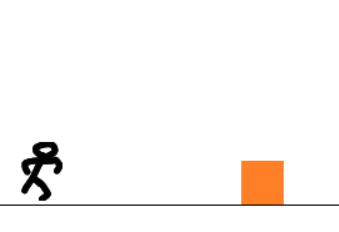
\includegraphics[width=2cm, height=2cm]{1b2.png}}\hfill
        \subfloat[]{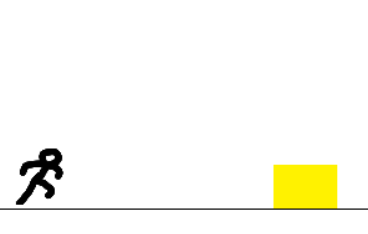
\includegraphics[width=2cm, height=2cm]{1b3.png}}\hfill
        \\
        \subfloat[]{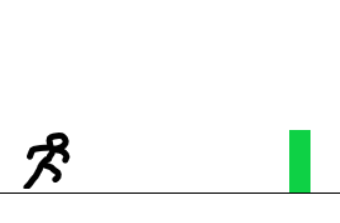
\includegraphics[width=2cm, height=2cm]{2b1.png}}\hfill
        \subfloat[]{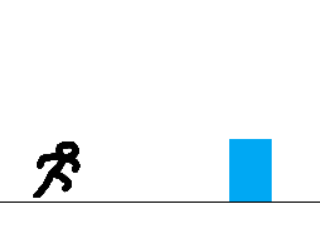
\includegraphics[width=2cm, height=2cm]{2b2.png}}\hfill
        \subfloat[]{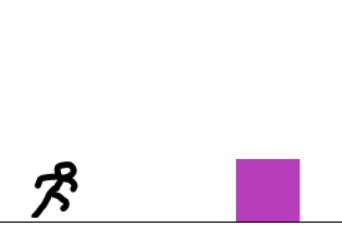
\includegraphics[width=2cm, height=2cm]{2b3.png}}\hfill
        \\
        \subfloat[]{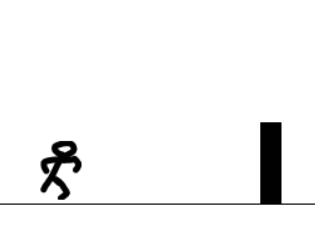
\includegraphics[width=2cm, height=2cm]{3b1.png}}
   \end{center}     
\caption{Seven Different Obstacles in the Game}    
\end{figure}

\subsection{Fitness Function}
To compute for the fitness of the agent, two components are used:
\begin{itemize}
\item Traveled Distance (TD): a counter that increases in every interaction of the agent to the environment
\item Score: the number of obstacles already transposed
\end{itemize}

These two component are then combined to form our fitness function
$$
 FitnessFunction = Score + (TD*0.001) 
$$
This function shows that the fitness of the agent is a linear combination of the score and the travelled distance which is regulated by 0.001 to not overpower the importance of the score in the function.

The goal of the agent is then to travel the
maximum possible distance and to obtain the highest score set

\subsection{NEAT-Python Set Up and Training Settings}

In this work, the Neuroevolution of augmenting topologies (NEAT) python library was used to create the Artificial Neural Network for each individual in the population which served as its brain to decide on its interaction to the game environment. Additionally, the NEAT python library was used to evolve the Artificial Neural Networks by following the NEAT algorithm which involves:

\begin{itemize}
\item Fitness Calculation: Each individuals will be evaluated according to their fitness using the fitness function
\item Elitism: The process of preserving the specified amount of top genomes in a specie with respect to their fitness level. The non selected genomes will be culled
\item Crossover: The process of producing offspring from those who survived elitism for repopulation of genomes.
\item Mutation: The process of randomly adding or removing nodes or connections to a randomly selected genome. The weights and Bias of the genome are also randomly mutated to a specified ratio.
\end{itemize}

An overview of the NEAT algorithm can be seen in Figure 6.

\begin{figure}[htbp]
\begin{center}
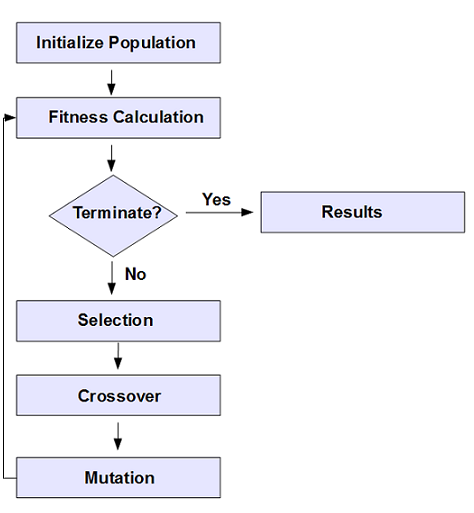
\includegraphics[width=8cm, height=6cm]{GAprocess.png}
\caption{Flowchart for NEAT}
\end{center}
\end{figure}

In the configuration of the NEAT parameters, the following
values were established:
\begin{itemize}
\item Population: a population of 30 is used. It is small enough for faster execution and is large enough to allow a genomic diversity.
\item Elitism: an elitism of 2 individuals per specie was chosen. This value allows the preservation of innovations and it is small enough to not incur stagnation or the absence of innovations.
\item Compatibility threshold: the value given to this term is 3.0, which is large enough to not create many species initially and is small enough to not completely prevent the formation of species within the population.
\item Probabilities to add or remove connections: the likelihood
of adding connections and removing connections were set to 0.2 and 0.2 respectively. This causes to change the topology not immediately but gradually, since NEAT starts from less complex to more complex topologies.
\item Probabilities to add or remove nodes: the likelihood
of adding nodes and removing nodes were set to 0.2 and 0.2, as in the above parameters, and they have a similar explanation.
\item Bias Mutate Rate and Replace Rate: the chance of the bias of node to mutate and to be replaced were set to 0.7 to 0.1 respectively. This causes slight changes to the output of the artificial neural network, thus allowing different behaviors for the game agent to display with a possibility of finding the solution for the game.
\item Weight Mutate Rate and Replace Rate: the chance of the weight of a connection to mutate and to be replaced were set to 0.8 to 0.1 respectively. The purpose is as same as stated above parameters.
\end{itemize}

The NEAT algorithm using sigmoid as an activation function was run for 30 times in which the maximum generation allowed is set to 30 and the maximum fitness cap of about 50 scores or 50 obstacles to be transposed.

\section{RESULTS and DISCUSSIONS}

\subsection{NEAT Run Trials}
After a trials of 30 runs, the NEAT algorithm has successfully produced an game agent that has breached 50 obstacles on 25 of those runs. In other words that the experiment has shown a success rate of about 83.33 percentage. The generations in which the breakthrough has occurred and its frequency can be seen on Figure 7. The data available in the chart was used to acquire the average generation wherein a successful game agent can be produced which is at 16.8 generation.

\begin{figure}[htbp]
\begin{center}
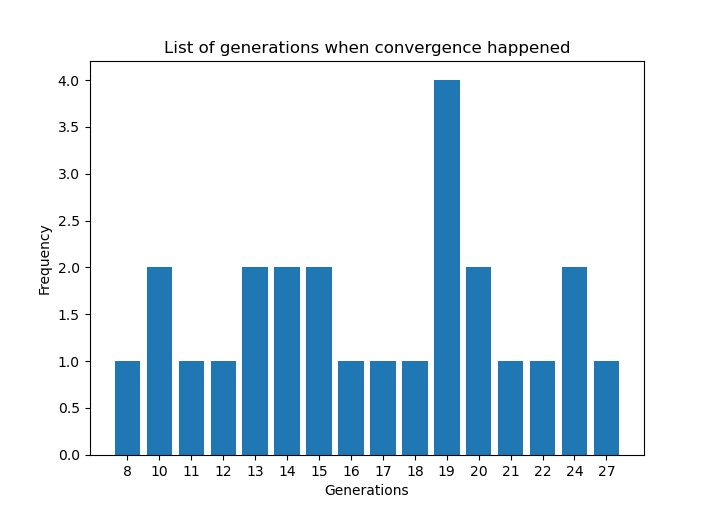
\includegraphics[width=8cm, height=6cm]{genPlot.png}
\caption{Generation x Frequency Success Training}
\end{center}
\end{figure}

\subsection{Genome Features Scaling and Importance}
Succeeding every experiments runs was the recording of the final population with 30 individuals, in which after 30 trials would bring it to a total of 900 individuals documented. Shown in Figure 8 are the average weight inputs which are classified to their own type of input with respect to their fitness. Moreover, the zero average input weights indicates that the respective input type it belongs to is currently inactive, or in other words they are unimportant. 

\begin{figure}[htbp]
\begin{center}
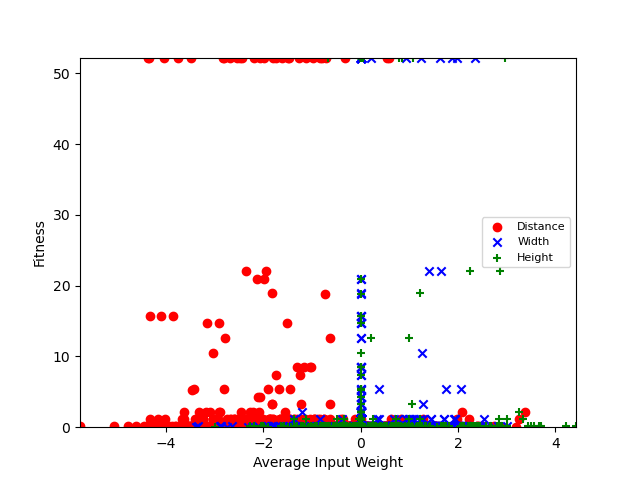
\includegraphics[width=8cm, height=6cm]{scatterPlot.png}
\caption{Average Input Weights x Fitness}
\end{center}
\end{figure}

Each of the 900 individuals has 3 inputs which signifies that there are also 900 average weights for each of the 3 types of input. In those 900 average weights there are about 764 activated average weight input for the distanceInput, while there are 322 activated average weight input for the widthInput. Lastly, there are 237 activated average weight input for the heightInput. This implies that after running the experiment, the NEAT algorithm has decided that the distanceInput is the most important input for all the genomes while the widthInput follows behind with the heightInput taking the last.

Among the 900 individuals recorded after the experiment, only 28 individuals has managed to transpose 50 obstacles. Shown in Figure 9 are the distribution of the average input weights of the 28 individuals who has passed the trials. It can be seen that the most active input type is the distanceInput, in which all 28 are activated with 26 are on negative scale while 2 are on positive scale. Meanwhile both the widthInput and heightInput are almost nonexistent with merely 7 active average weight input which are all on the positive scale for the widthInput while there are 6 activated weight input for the heightInput which is 1 for negative scale and 5 for the positive scale. This signifies that even among the individuals who has passed the experiment, the distanceInput is still more influential compared to the other two input type.

\begin{figure}[htbp]
\begin{center}
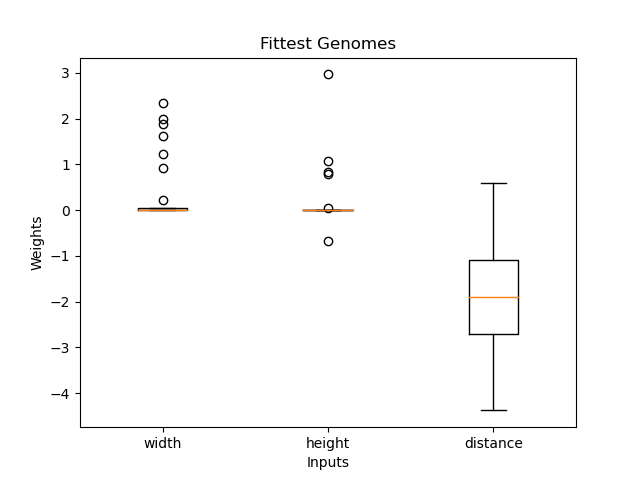
\includegraphics[width=8cm, height=6cm]{fitPlot.png}
\caption{Distribution of Average Weight inputs of fittest genomes}
\end{center}
\end{figure}

Additionally, the dominant negative polarity of the average weight input of distanceInput indicates that it is inversely proportionate to the output of the topology. It means that the negative weight of the distanceInput ensures that when the agent has a high value of Distance to Obstacle, the sigmoid function will tend to result in a very low jump probability. This implies that the agent will tend to not jump when the obstacle is still far. However, when the agent has a low Distance to Obstacle, the sigmoid function will tend result in a very big jump probability, which will lead the agent
jump up when obstacles are near.

\section{CONCLUSION}
In this work, the author proposed the use of Neuroevolution of Augmenting Topologies (NEAT) algorithm for evolving and to generate an artificial agent capable of achieving optimal scores in the Modidified Stick Running. By using only 30 individuals, the NEAT algorithm was run for 30 trials with a maximum of 30 generations per trial. The NEAT algorithm was able to produce an individual that has breached the maximum specified score of 50 with a success rate of 83.33 percentage and an average of breakthrough at 16.8 generations. After the experiment, the NEAT algorithm has designated that the distanceInput as the most important input amongst the other which included the widthInput and heightInput. Additionally, the NEAT algorithm has put heavy importance on designating negative weight inputs for the distanceInput to ensure inverse proportionality to the output. It ensures that the game agent will jump much proficiently whenever an obstacle is near it. Overall, this shows that the NEAT algorithm can be used to create an artificial game agent capable of playing the Modified Stick Running.

For future works, the NEAT algorithm can also be used on other simple platform game. Additionally, you can also add another algorithm alongside the NEAT algorithm in producing game agent for this game or another simple platform game.

\begin{thebibliography}{99}

\bibitem{c1} K. O. Stanley and R. Miikkulainen. Evolving Neural Networks Through Augmenting Topologies. Evolutionary Computation, 10(2):99-127, 2002.

\bibitem{c2} K. O. Stanley and R. Miikkulainen. Evolving neural networks through augmenting topologies. Technical Report AI01-290, The University of Texas at Austin, Department of Computer Sciences, June 1 2001. Mon, 28 Apr 103 21:15:41 GMT.

\bibitem{c3} E. Guizzo, “How googles self-driving car works”. IEEE Spectrum Online, October, 18, 2011.

\bibitem{c4} J. E. Laird. “Using a computer game to develop advanced AI”. Computer, 34(7):70-75, 2001.

\bibitem{c5} L. Galway, D. Charles and M. Black. Machine learning in digital games: A survey. Artif. Intell. Rev.. 29. 123-161. 10.1007/s10462-009-9112-y, 2008.

\bibitem{c6} G. Tesauro. Temporal difference learning and td-gammon. Communications
of the ACM, 38(3):5868, 1995.

\bibitem{c7} V. Mnih, K. Kavukcuoglu, D. Silver, A. A. Rusu, J. Veness, M. G. Bellemare, A. Graves, M. Riedmiller, A. K. Fidjeland, G. Ostrovski, S. Petersen, C. Beattie, A. Sadik, I. Antonoglou, H. King, D. Kumaran, D. Wierstra, S. Legg, and D. Hassabis. Human-level control through deep reinforcement learning. Nature, 518(7540):529–533, 2015.

\bibitem{c8} M. G. Bellemare, Y. Naddaf, J. Veness, and M. Bowling. The arcade learning environment: An evaluation platform for general agents. arXiv preprint arXiv:1207.4708, 2012.

\bibitem{c9} K. O. Stanley and R. Miikkulainen, “Evolving a roving eye for go,” in Proceedings of the Genetic and Evolutionary Computation Conference (GECCO-2004). Berlin: Springer Verlag, 2004.

\bibitem{c10} K. O. Stanley, B. D. Bryant, and R. Miikkulainen, “Real-time neuroevolution in the NERO video game,” IEEE Trans. Evol. Comput., vol. 9, no. 6, pp. 653–668, 2005.

\bibitem{c11} E. J. Hastings, R. K. Guha, and K. O. Stanley, “Automatic content generation in the galactic arms race video game,” IEEE Transactions on Computational Intelligence and AI in Games, vol. 1, no. 4, pp. 245–263, Dec 2009.

\bibitem{c12} T. Kristo and N. U. Maulidevi, “Deduction of fighting game countermeasures using neuroevolution of augmenting topologies,”
in 2016 International Conference on Data and Software
Engineering (ICoDSE), Oct 2016, pp. 1–6.

\bibitem{c13} J. Schrum and R. Miikkulainen, “Discovering multimodal behavior in ms. pac-man through evolution of modular neural networks,” IEEE Transactions on Computational Intelligence and AI in Games, vol. 8, no. 1, pp. 67–81, March 2016.

\bibitem{c14} Github, [Online] https://github.com/CodeReclaimers/neat-python

\bibitem{c15} Github, [Online] https://github.com/pygame/pygame
 
\end{thebibliography}

\begin{wrapfigure}{l}{25mm}
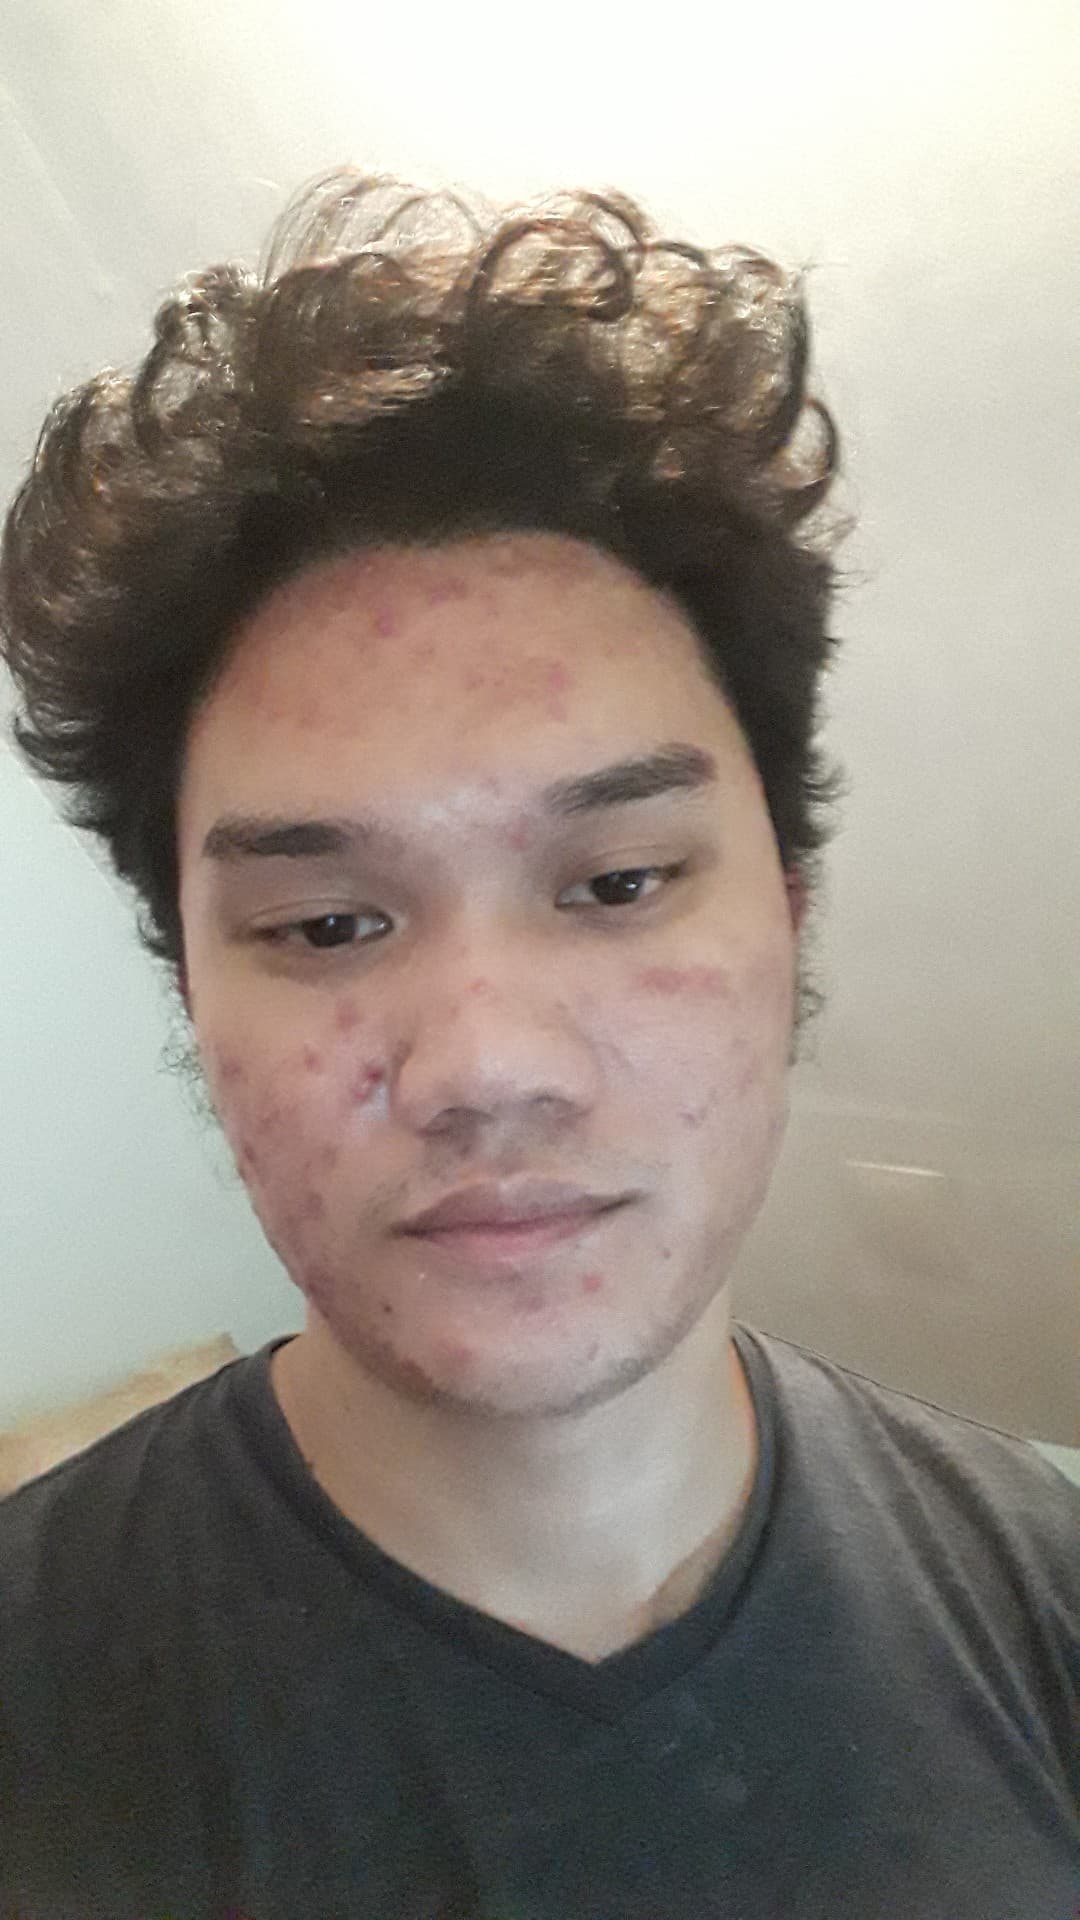
\includegraphics[width=1in,height=1.25in,clip,keepaspectratio]{selfie.jpg}
\end{wrapfigure}\par

   \textbf{Aldrich S. Goco} son of Helen S.Goco and Leo P. Goco is a BS Computer Science undergraduate student of the University of the Philippines Los Banos. He loves to spend most of his time on reading light novels and watching youtube recommendations varying from war history, conspiracy theories, video games, bodybuilding and much more

\end{document}
